%% We use `subfiles' package
\documentclass[preamble.tex]{subfiles}
\begin{document}

\clearpage

\chapter{Delaying array computations}

This chapter describes \LiveFusion - the new array language that I designed. It offers a library of fusible array combinators and is able to exploit more fusion opportunities than equational fusion frameworks\ieqfusion (see Appendix \ref{sec:Equational-Fusion-Systems})

In its essence \LiveFusion takes the approach of \*deeply embedded domain specific languages* (EDSLs).\iedsl


\section{On Embedded Domain-Specific Languages}
\iedsl

The term \term{domain-specific language} (DSL) describes a computer language designed for solving problems in a particular application domain.

Examples of DSLs include \name{HTML} for webpages markup \cite{HTML}, \name{SQL} for relational database queries \cite{SQL} and \name{Verilog} for hardware description \cite{Verilog}.

In contrast, \Haskell \cite{Pey03} is a \*general purpose language* and is more widely applicable across domains.

On the other hand, an \term{embedded domain-specific language} (EDSL) is a domain-specific language which is designed to be used from within another language, called \*host* language. It is implemented as a library for the host language and can reuse its syntax, compiler and the runtime system.

The added benefit of the approach is that the EDSL code can interact with the rest of the code in the host language. This way the programmers do not have to leave the familiar environment and can write EDSL programs which are seamlessly integrated with their programs.

Two types of embedding exist:
\begin{description}
\item \term{Shallow embedding}

Shallowly embedded DSLs directly translate their constructs to expressions in the host language. They offer a fixed interpretation of their operations.

\name{Parsec}\footnote{parsec: Monadic parser combinators - http://hackage.haskell.org/package/parsec} library of parsing combinators is an example of a shallow EDSL for \Haskell.

\item \term{Deep embedding} 

The principle idea behind \term{deeply embedded DSLs} is that all operations of such an EDSL construct a tree of operations, or an \term{abstract syntax tree} (AST).\iast This new AST is a data structure in the host language. It is separate from the host language's AST and is rather presented as a tree-like structure in the host language's runtime.

The difference from the ASTs found in compilers is that it allows for analysis, optimisation and compilation (or interpretation) of the EDSL's AST at runtime. The complete process is taken care by the library written in the host language. This avoids the difficulties of writing a complete standalone optimising compiler.

\name{Accelerate} language for functional programming on GPUs \cite{CKL+11} is a vivid example of a deeply embedded DSL.
\end{description}

\LiveFusion EDSL falls under the category of deeply embedded domain-specific languages. In this chapter I describe the process of embedding array computations.


\clearpage

\section{LiveFusion AST}

\LiveFusion EDSL offers a library of flat and segmented\isegmented array combinators\icomb some of which are presented in Listing \ref{lst:LiveFusion-interface}.

\begin{hscode2}[%
    caption={\LiveFusion interface functions. Typeclass constraints on array elements have been omitted for brevity.},%
    label=lst:LiveFusion-interface,%
]
type Array a = ArrayAST a

-- * Flat array combinators
map      :: (Term a -> Term b) -> Array a -> Array b
filter   :: (Term a -> Term Bool) -> Array a -> Array a
zipWith  :: (Term a -> Term b -> Term c) -> Array a -> Array b -> Array c
zip      :: Array a -> Array b -> Array (a,b)
fold     :: (Term a -> Term a -> Term a) -> Term a -> Array a -> a
scan     :: (Term a -> Term a -> Term a) -> Term a -> Array a -> Array a

-- * Segmented array combinators
scan_s   :: (Term a -> Term a -> Term a) -> Term a
         -> Array Int -> Array a -> Array a
fold_s   :: (Term a -> Term a -> Term a) -> Term a
         -> Array Int -> Array a -> Array a
\end{hscode2}


\begin{hscode2}[%
    caption={\LiveFusion AST (partial).},%
    label=lst:LiveFusion-AST,%
]
type ArrayAST a = AST (Vector a)
type ScalarAST a = AST a

data AST t where
  Map      :: (Elt a, Elt b)
           => (Term a -> Term b)
           -> ArrayAST a
           -> ArrayAST b

  Filter   :: Elt a
           => (Term a -> Term Bool)
           -> ArrayAST a
           -> ArrayAST a

  Fold     :: Elt a
           => (Term a -> Term a -> Term a)
           -> Term a
           -> ArrayAST a
           -> AST a

  Scan     :: Elt a
           => (Term a -> Term a -> Term a)
           -> Term a
           -> ArrayAST a
           -> ArrayAST a

  Scan_s   :: Elt a
           => (Term a -> Term a -> Term a)
           -> Term a
           -> ArrayAST Int
           -> ArrayAST a
           -> ArrayAST a

  Manifest :: Elt a
           => Vector a
           -> ArrayAST a
\end{hscode2}

The fundamental concept by which \LiveFusion makes fusion possible is constructing an AST\iast of pending array operations at runtime and compiling that AST to fast code when the result is required in the host program. By constructing an AST of a pipeline of array operations in a running program, the actual computations are \*delayed* to be performed at a later time.

The AST is the topmost layer of \LiveFusion system. Most of the library's user-facing functions are just constructing the nodes of the AST. Parts of \LiveFusion AST are presented in Listing \ref{lst:LiveFusion-AST}. Is it easy to spot the correspondence between the user-facing functions in Listing \ref{lst:LiveFusion-interface} and the constructors of the AST.

\LiveFusion AST is a \*Generalised Algebraic Data Type* (GADT) \cite{Jones:2006eh} whose individual constructors correspond to delayed array operations.

In principle, given an interpreting function such as @eval :: AST t -> t@, a value of type @t@ encoded in the @AST@ language can be computed.Notably, @t@ in @AST t@ is not necessarily an array. In fact we know not all of the array combinators return an array: in particular @fold@ and several others return a scalar value.

\section{LiveFusion EDSL by example}

I will now present a simple user program that can be written using \LiveFusion library. Listing \ref{lst:farAndAbove} presents the core of the QuickHull algorithm. The corresponding runtime AST for the same function is given in Figure \ref{fig:QuickHull-flat}.

\todo{TODO}
\textsc{TODO: Offer a simple flat version of QuickHull and elaborate it into a proper segmented one. Aternatively give dotp as example.}

\begin{hscode2}[%
    caption={\code{farAndAbove} function, core of QuickHull.},%
    label=lst:farAndAbove,%
]
farAndAbove :: (Point,Point) -> Array Point -> (Array Point, Point)
farAndAbove line points
  = let distances = map (dist line) points

        -- Find maximum point
        indexed     = zip (indices distances) distances
        farthest_ix = fst $ fold maxSnd 0 distances
        farthest    = points ! farthest_ix
        maxSnd x y  = if snd x >. snd y
                      then x
                      else y

        -- Find all points above the line
        positive    = map (>. 0) distances
        above       = packByTag positive points

    in  (above, farthest)
\end{hscode2}

\begin{figure}
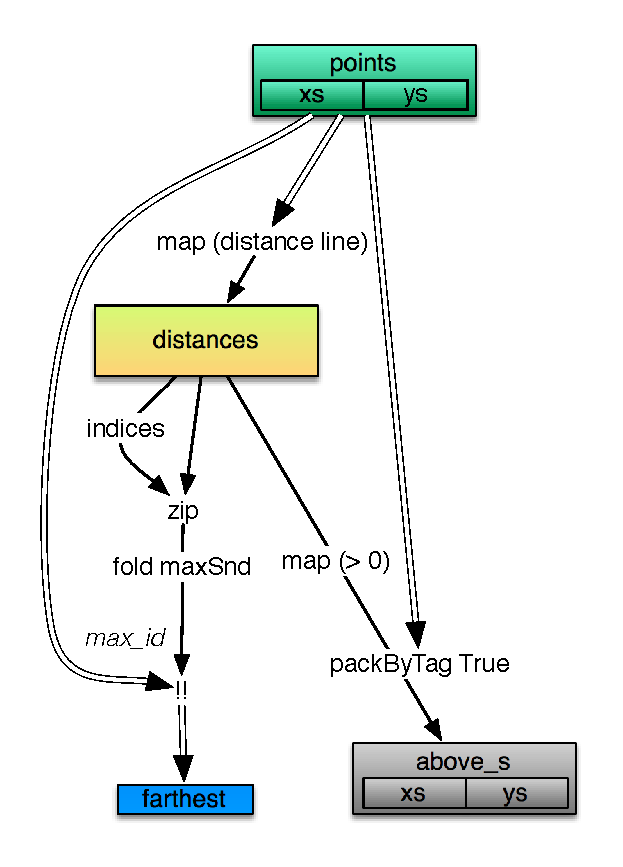
\includegraphics[width=0.4\textwidth,center]{img/QuickHull-flat-but-true}
\caption{\label{fig:QuickHull-flat}{AST for the core of QuickHull example: arrow labels are AST nodes, coloured boxes are potentially manifest arrays.}}
\end{figure}

%The above example uses six array combinators: @map@, @zip@, @indices@, @pack@, @fold@ and the indexing combinator @(!!)@. The first four of them are \*array transducers* in that they both consume and produce arrays. On the other hand @fold@ and @(!!)@ consume arrays and return a scalar value, so we call them pure consumers.

%It is now time to show the AST node constructors these combinators correspond to. 


\section{Parametrising higher-order combinators}
\label{sec:Scalar-language}
\iscalarlang

Another notable feature of the interface to note here is the type of functions that parametrise higher-order combinators:

\begin{hscode}
map    :: (Term a -> Term b) -> Array a -> Array b
filter :: (Term a -> Term Bool) -> Array a -> Array Bool
\end{hscode}

The corresponding Haskell list functions or array libraries like @Vector@ or @Repa@ \cite{KCL+10} accept as arguments vanilla Haskell functions like @a -> b@ or @a -> a -> a@ as long as the types match.

The question that should be asked, however, is why cannot \LiveFusion do the same?

%\LiveFusion AST is open to interpretation by several backends as discussed in Chapter \ref{ch:Code-Generation}.
The answer lies in the approach to evaluating the AST. In order to be efficient the AST needs to be compiled into highly optimised code. During compilation (discussed in Chapter \ref{ch:Code-Generation}) the AST is compiled to one or more loops for which Haskell code is generated and written out to file.

If the parametrising functions were simple Haskell functions, they would have been compiled to machine code before the program is run. When the AST is later constructed at runtime they would only be available in the form of closures which can be called but not inspected\footnote{There is a non-portable way to explore closures in Haskell, but it will not allow one to easily make use of the code compiled to binary.}.

Suppose the user writes @map (+1) xs@. The function @(+1)@ needs to be inlined into the compiled loop code to produce efficient code. If this does not happen, calling @(+1)@ for every element in the array will result in the following:

\begin{enumerate}
\item Boxing the element value by placing it in the heap
\item Calling the closure with the pointer to the boxed value
\item Jumping to the address of the @(+1)@ function referenced in the closure
\item The code will unbox the value, increment it and create a new value on the heap
\item The loop code will then need to unbox the result and write it into the result array
\end{enumerate}

This is a very round-about way of incrementing a value in a tight loop and will greatly affect the performance of the loop.

Unfortunately, at the time of generating code for AST, all these Haskell functions will have been compiled to machine code and are only available as closures. There is currently no way to inline them or reify them into the original Haskell source code from which they were created.

I needed to find a way to generate efficient code for user specified functions at runtime. I needed a way to record the user-provided functions in a more high level way than machine code.

In summary the chosen representation for functions:
\begin{enumerate}
\item Provides backend independent interface offering many common functions
\item Allows backend-specific implementation for each function
\item Hides implementation from the user by default
\item Allows user to compose functions in a way that looks native
\item Allows user to provide direct backend-specific implementation for new functions that cannon be composed from functions already provided
\end{enumerate}

The following section explains how this is achieved.

\subsection{Scalar Term language}

So what is an expression of type @Term a -> Term b@?

It is a term in our scalar expression language \name{Term}, representing a function from type @a@ to type @b@. The AST for the \name{Term} language is given in Listing \ref{lst:HOAS}.

\begin{hscode2}[%
    caption={Term language for HOAS representation.},%
    label=lst:HOAS,%
]
data Term t where
  -- Function or constant in backend-specific form
  Con :: Impl t -> Term t

  -- Lambda abstraction
  Lam :: (Term s -> Term t) -> Term (s -> t)

  -- Function application
  App :: Term (s -> t) -> Term s -> Term t

  -- for conversion to de Bruijn representation
  Tag :: Level -> Term t

type Level = Int
\end{hscode2}

This simple language allows to represent the user to write functions in the higher-order abstract syntax (HOAS) form. The user could write function in a familiar form\footnote{The above code assumes that \code{Term Int} is in the type class \code{Num}}:

\begin{hscode}
f :: Term Int -> Term Int
f x = x * x + 1
\end{hscode}

\todo{talk HOAS}


\subsection{Backend specific function implementations}

One notable part of the @Term@ language is its @Con@ constructor. The only argument to the constructor is @Impl t@ offers a backend-dependent way of to define a function. @Impl@ data type gives freedom to the backend to choose the most suitable representation for a function.

For instance, in the \Haskell backend for \LiveFusion we are interested in generating \Haskell source code, for which \name{Template Haskell} \cite{TH} is a natural choice. Thus we choose the following definition of @Impl@:

\begin{hscode}
data Impl t = HsImpl {
                hs :: t,        -- Native Haskell function
                th :: Q TH.Exp  -- TemplateHaskell quasiquoted expression
              } 
\end{hscode}


The \name{Template Haskell} expression is really the core part of the function representation, but this is what would later on allow for an easy production of \Haskell source code at the code generation stage.

The representation also includes the vanilla \Haskell function. At present this is just for completeness. However in the future it may be possible to avoid compiling certain parts of AST at runtime and run statically scheduled combinators. In this case this would be the function to inline into the loop.

We will now see the (rather trivial) implementations for a couple of functions before continuing with our explanation of Impl.

\begin{hscode}
plusImpl :: Num a => Impl (a -> a -> a)
plusImpl = HsImpl { hs = (+); th = [| (+) |] } 

absImpl :: Num a => Impl (a -> a)
absImpl = HsImpl { hs = abs; th = [| abs |] } 
\end{hscode}

It is easy to see that \name{Template Haskell} expressions are trivially created from simple Haskell functions using \name{quasi-quotation} extension \cite{QQ}.

When the backend is ready to generate \Haskell source for these functions, it will be a simple matter of using a \name{Template Haskell's} pretty printer. 

The reasons for using \name{Template Haskell} expressions (is the following):
\begin{itemize}
\item The backend does non-trivial code generation as discussed in Chapter \ref{ch:Code-Generation}, where the full power of \name{Template Haskell} is required. Functions defined this way become very easy to incorporate into the generated code
\item New developments in \name{Template Haskell}\footnote{Starting with GHC 7.8.} will allow its expressions to be typed. Having @Q (TExp t)@ as opposed to @Q Exp@ will provide an extra layer of safety to our function representation
\end{itemize}

\todo{Perhaps show how a function is passed to the AST using lam and app.}
\todo{subsection{Function composition}}

\subsection{User-defined implementation of parametrising functions}

The library provides backend-specific implementations for many standard functions including all of the functions from such type classes as @Num@, @Floating@, @Ord@-like and @Eq@-like, as well as a the ability to compose them into more complex functions.

However, the flexibility of the library does not end there. One feature of the given scalar functions representation is that it allows the user of the library to define new functions. After all, it only requires creating a new record of type @Impl t@ where @t@ is the type of the desired function. Library user can then provide the internals of function implementation to appear in the generated code.

This leaves the door open to the user and makes the library more flexible and extensible.

%% The following discussion is excluded from the document
\begin{comment}
\section{On the flexibility of parametrising functions}

\begin{itemize}
\item Currently function representation of only one backend was shown, namely Haskell source backend.
\item Even that one was trivial: only containing a TH Exp + native HS function
\item What other functionality may we want in our function representation?
\item LiveFusion is a fast array processing library. The focus is on performance.
\item Our two main options for speed on modern CPUs: parallelism + vector instructions.
\item Parallelism is already exploited by DPH through other means and will split the computations evenly across all cores
\item Vectorisation on the other hand has not been exploited by DPH yet\footnote{Though new developments in that area have emerged more recently \todo{ref}}
\item The CPU manufacturers are introducing and announcing more and more vector instruction sets\footnote{\todo{ref}: Intel Future Instruction Sets} which will allow many types of vector operations to be performed on each core.
\item This is very handy for libraries like LiveFusion which are already providing patterns of array computation, some of which map very well to vector instructions of current or future CPUs \todo{find examples, but this will definitely include point-wise arithmetic, reductions and pack}.
\item At some point in the future @Impl@ function representation may be the most natural place to include backend- or even CPU-specific information, on how to generate vector instructions for a particular function, e.g. a reduction using product operator on an Intel CPU.
\end{itemize}

\end{comment}

\begin{comment}
\section{Compiling Delayed LiveFusion AST}

\section{Sharing recovery: Abstract Semantic Graphs}

\begin{itemize}
\item Begin with Oleg's blessing quote. On two probs.
\item Find example, should be plenty in QuickHull
\item Talk about ref transparency of Haskell
\item Two types of sharing really, talk shapes
\item While can still fuse, it performs unnecessary work
\item Implicit vs. explicit sharing (ref email thread)
\item For implicit:
\item Still represented by the same object internally at runtime
\item StableNames, Gill's, but can do other, pointer equality sharing recovery
\item It's is IO, but since we are in a library and can guaranty safety by design we don't care
\end{itemize}
\end{comment}

\IfNotCompilingAll{\bibliography{bib}}

\end{document}